\documentclass[12pt]{article}
\usepackage[a4paper, total={6in, 9in}]{geometry}
\usepackage{graphicx}
\graphicspath{ {./images/output/} }
\usepackage{caption}
\usepackage[english]{babel}
\usepackage{titling}
\usepackage{float}
\usepackage{amsmath}
\usepackage{minted}
\usepackage{multicol}
% \usepackage{makecell}
\usepackage{tabularx}
\usepackage{multirow}
\usepackage{adjustbox}
% \usepackage{array}
% \usepackage{setspace}
% \usepackage{placeins}
\setlength{\parindent}{0pt}

% \usepackage{lipsum}

\title{Study of Pulse Code Modulation (PCM)}
\author{}
\date{}

\pagenumbering{gobble}
\begin{document}
\vspace*{\fill}
\begin{center}

    \emph{Heaven's Light is Our Guide} \\
    \textbf{Rajshahi University of Engineering and Technology} \\

    \begin{figure}[H]
        \centering
        
\includegraphics[scale=.34]{images/RUET_logo.png}
        \label{fig:ruet_logo}
    \end{figure}
    \vspace{5mm}

    \textbf{Course Code}\\
    ECE 3208\\
    \vspace{3mm}
    \textbf{Course Title}\\
    Communication Engineering Sessional

    \vspace{5mm}
    \textbf{Experiment Date:} {January 21, 2025},\\
    \textbf{Submission Date:} {February 11, 2025}\\

    \vspace{5mm}
    \textbf{Lab Report 3: \\
        Determination of Modulation Index of FM Wave}

    \vspace{15mm}

    \begin{tabular}{c|c}
        \textbf{Submitted to} & \textbf{Submitted by} \\
        Dr. Md. Kamal Hosain  & Md. Tajim An Noor     \\
        Professor             & Roll: 2010025         \\
        Dept of ETE, RUET     &                       \\
    \end{tabular}

\end{center}
\vspace*{\fill}


\pagebreak

\tableofcontents

\pagebreak
\pagenumbering{arabic}
\maketitle

\section*{Theory}
\addcontentsline{toc}{section}{Theory}
Pulse Code Modulation (PCM) digitally represents analog signals, used in digital audio, telephony, and more. It involves sampling and quantization \cite{oppenheim1996signals}.

\subsection*{Sampling}
Sampling converts a continuous signal into discrete samples. According to the Nyquist-Shannon theorem, the sampling rate must be at least twice the highest frequency in the signal \cite{shannon1949communication}. Mathematically:
\[
    x[n] = x(nT_s)
\]
where \( T_s \) is the sampling interval.

\subsection*{Quantization}
Quantization maps sampled values to a finite set of levels, introducing quantization error. The quantized signal is:
\[
    x_q[n] = Q(x[n])
\]

\subsection*{Encoding}
Quantized values are encoded into binary form. The number of bits used determines the resolution \cite{proakis2007digital}.

\subsection*{Advantages of PCM}
\begin{itemize}
    \item High noise immunity
    \item Efficient storage and transmission
    \item Compatibility with digital systems
\end{itemize}

\subsection*{Applications of PCM}
\begin{itemize}
    \item Digital telephony
    \item Audio recording
    \item Data communication
\end{itemize}

\section*{Required Apparatus}
\addcontentsline{toc}{section}{Required Apparatus}
\begin{itemize}
    \item DigitalModulationDemodulationKit (DL 3155M61)
    \item Oscilloscope
    \item ConnectingWires
    \item PowerSupply
\end{itemize}

\section*{Diagrams}
\addcontentsline{toc}{section}{Diagrams}
\subsection*{Block Diagram of PCM System}
\begin{figure}[H]
    \centering
    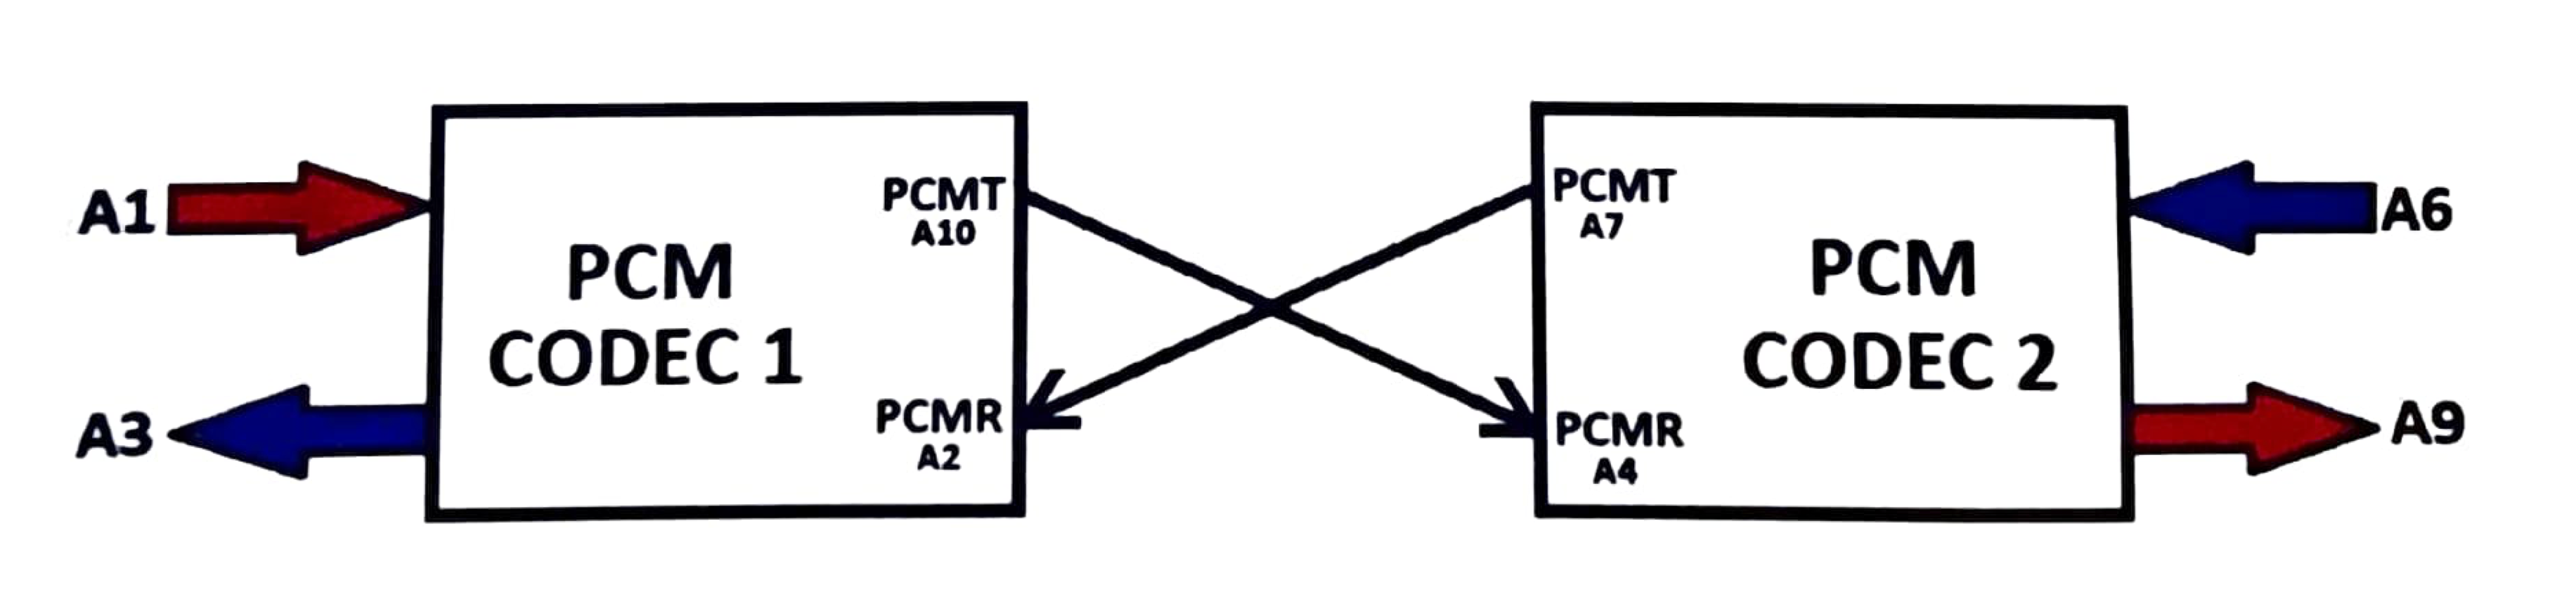
\includegraphics[width=\textwidth]{ckt.png}
    \caption{Block Diagram of PCM System}
    \label{fig:ckt}
\end{figure}

\begin{figure}[H]
    \centering
    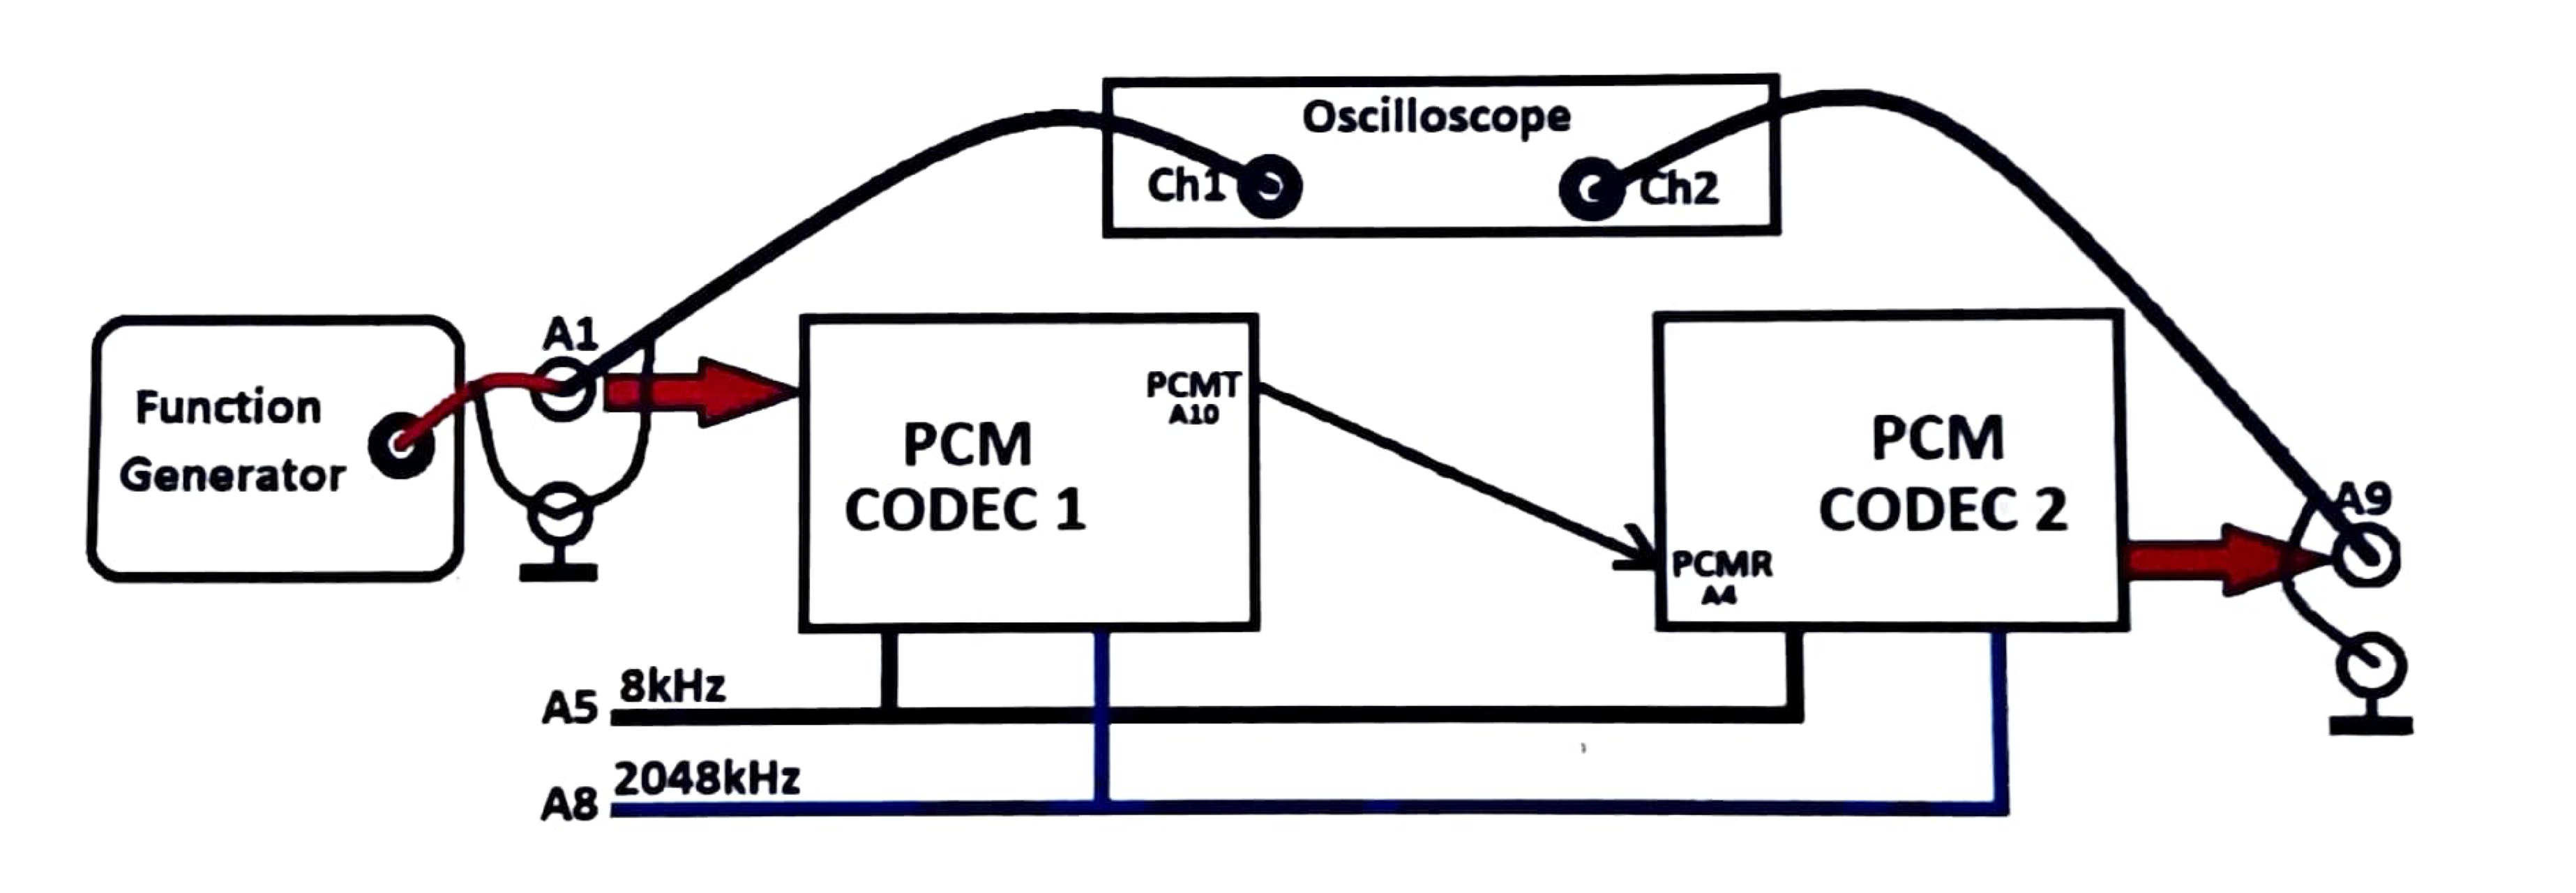
\includegraphics[width=\textwidth]{cktD.png}
    \caption{Block Diagram of PCM System (Detailed)}
    \label{fig:cktD}
\end{figure}

\subsection*{PCM Section of Kit DL 3155M61}
\begin{figure}[H]
    \centering
    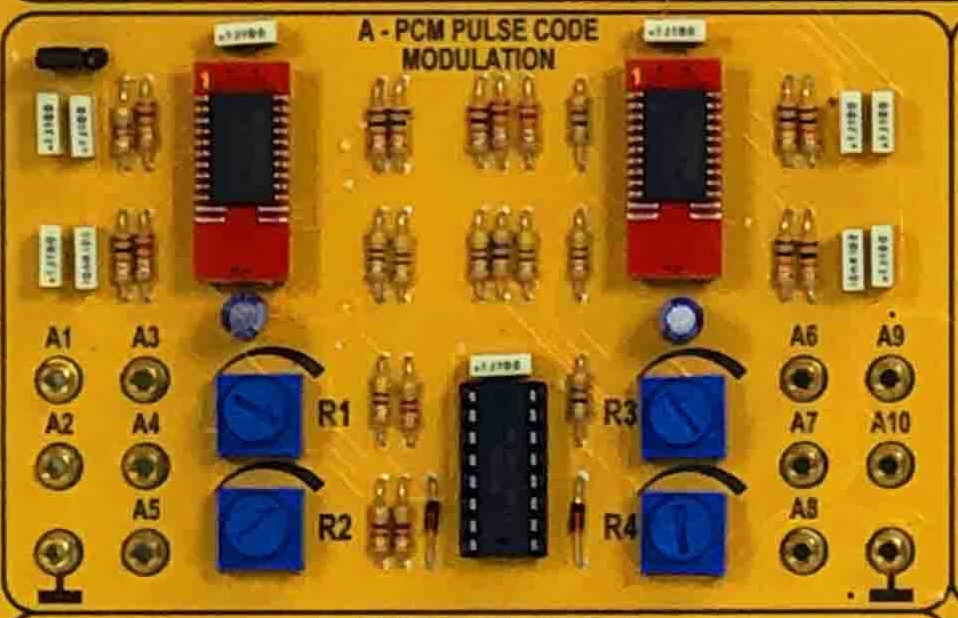
\includegraphics[width=.8\textwidth]{kit.jpg}
    \caption{PCM Section of Kit DL 3155M61}
    \label{fig:kit}
\end{figure}

\section*{Procedure}
\addcontentsline{toc}{section}{Procedure}
\begin{enumerate}
    \item The signal input (analog signal) was connected to pin A1.
    \item The PCM signal was observed on pins A10 and A4.
    \item The demodulated signal was observed on pin A9.
    \item Alternatively, the signal input was connected to pin A6.
    \item The PCM signal was observed on pins A7 and A2.
    \item The output signal was observed on pin A3.
    \item The 8kHz and 2048kHz signals were noted on pins A5 and A8.
    \item An oscilloscope was used to observe and verify the signals.
\end{enumerate}


% \section*{Experimental Data}
% \addcontentsline{toc}{section}{Experimental Data}

\section*{Observation}
\addcontentsline{toc}{section}{Observation}
We observed significant noise in the PCM and demodulated signals due to:

\begin{itemize}
    \item Faulty connections or components.
    \item External interference.
    \item Inaccurate sampling or quantization.
    \item Insufficient filtering of the analog signal.
\end{itemize}

Ensure secure connections, functional components, and proper shielding and filtering to reduce noise.


\section*{Matlab Simulation}
\addcontentsline{toc}{section}{Matlab Simulation}

\subsection*{Code:}
\addcontentsline{toc}{subsection}{Code}

\inputminted[linenos,breaklines,breakanywhere]{matlab}{./assets/pcm.m}

\section*{Output}
\addcontentsline{toc}{section}{Output}

\subsection*{Experimental Output}
\addcontentsline{toc}{subsection}{Experimental Output}
\begin{figure}[H]
    \centering
    \begin{minipage}{0.45\linewidth}
        \centering
        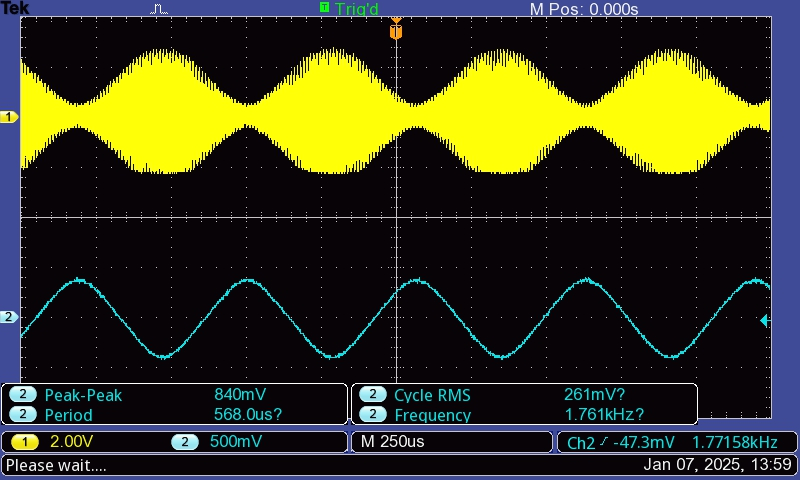
\includegraphics[width=\linewidth]{p1-undMod-msg.JPG}
        \caption{AM; Yellow: Under-modulated, Blue: Message}
        \label{fig:pic1}
    \end{minipage}
    \hfill
    \begin{minipage}{0.45\linewidth}
        \centering
        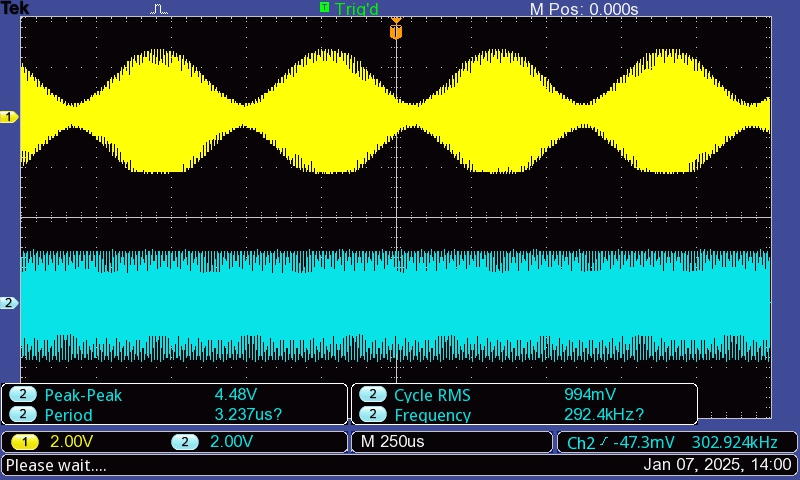
\includegraphics[width=\linewidth]{p2-undMod-car.JPG}
        \caption{AM; Yellow: Under-modulated, Blue: Carrier}
        \label{fig:pic2}
    \end{minipage}
    \vspace{1em}
    \begin{minipage}{0.45\linewidth}
        \centering
        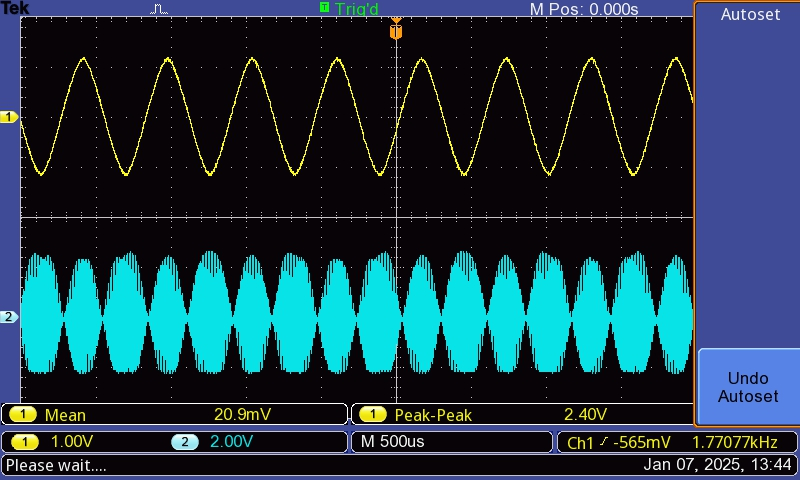
\includegraphics[width=\linewidth]{p3-msg-100mod.JPG}
        \caption{AM; Yellow: Message, Blue: 100\% Modulated}
        \label{fig:pic3}
    \end{minipage}
    \hfill
    \begin{minipage}{0.45\linewidth}
        \centering
        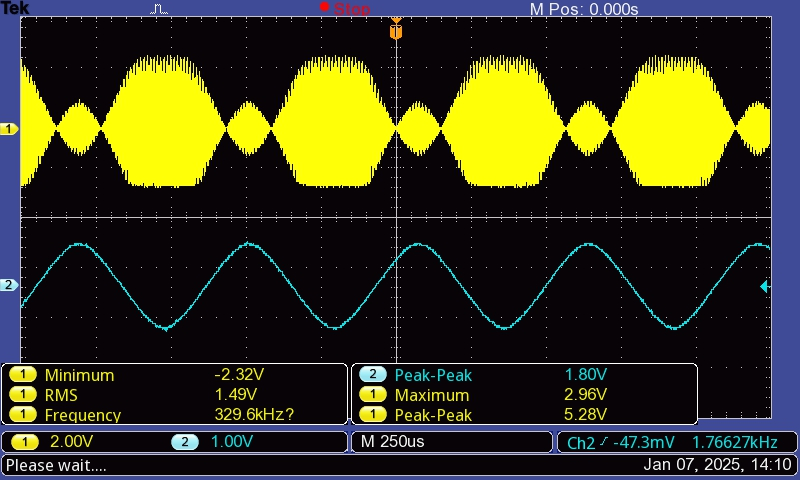
\includegraphics[width=\linewidth]{p4-ovMod-msg.JPG}
        \caption{AM; Yellow: Over-modulated, Blue: Message}
        \label{fig:pic4}
    \end{minipage}
    \vspace{1em}
    \begin{minipage}{0.45\linewidth}
        \centering
        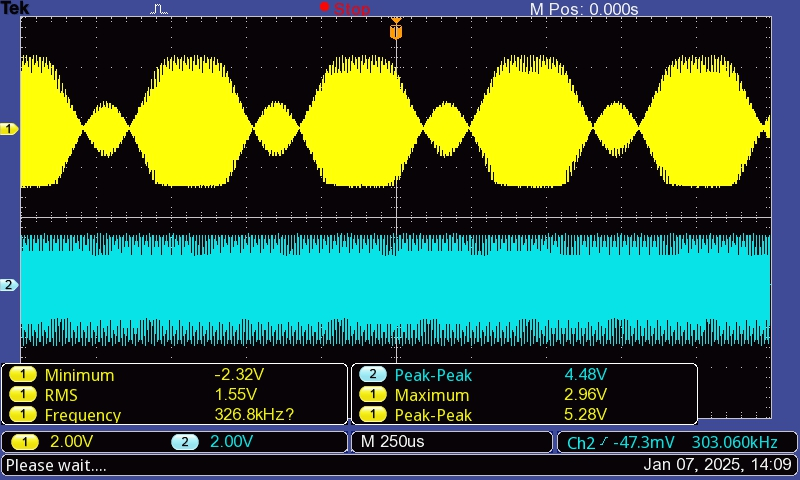
\includegraphics[width=\linewidth]{p5-ovMod-car.JPG}
        \caption{AM; Yellow: Over-modulated, Blue: Carrier}
        \label{fig:pic5}
    \end{minipage}
    \hfill
    \begin{minipage}{0.45\linewidth}
        \centering
        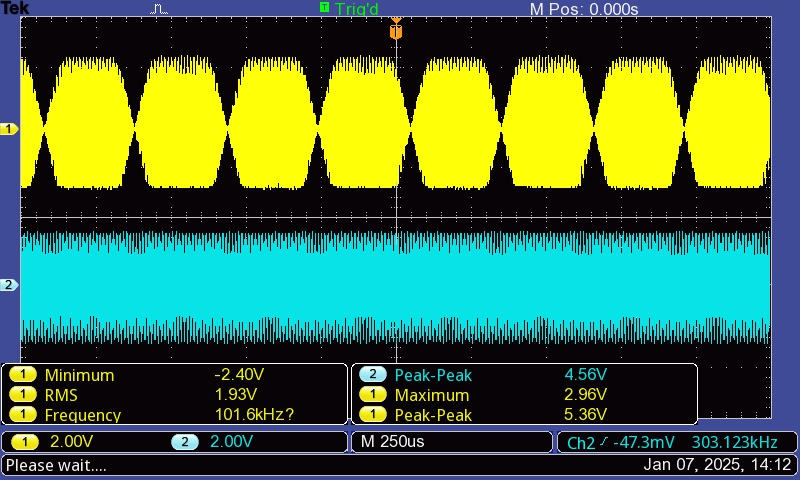
\includegraphics[width=\linewidth]{p6-dsb-mod-car.JPG}
        \caption{DSB\-SC; Yellow: Modulated, Blue: Carrier}
        \label{fig:pic6}
    \end{minipage}
\end{figure}

\pagebreak

\begin{figure}[H]
    \centering
    \begin{minipage}{0.45\linewidth}
        \centering
        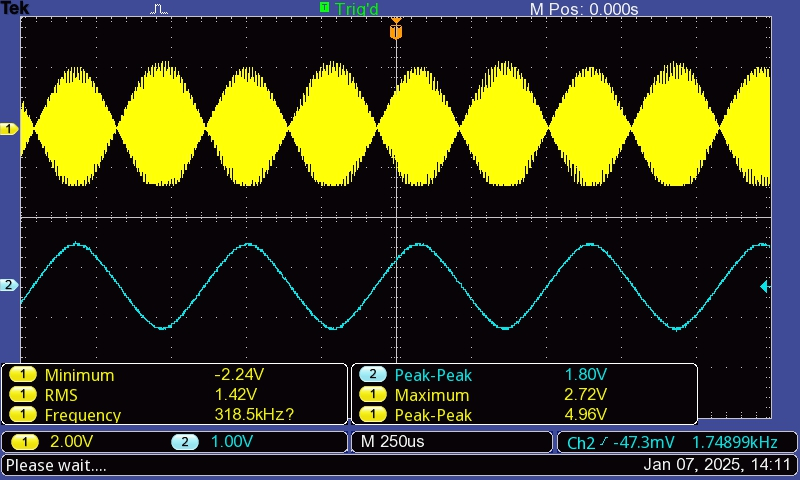
\includegraphics[width=\linewidth]{p7-dsb-mod-msg.JPG}
        \caption{DSB\-SC; Yellow: Modulated, Blue: Message 1}
        \label{fig:pic7}
    \end{minipage}
    \hfill
    \begin{minipage}{0.45\linewidth}
        \centering
        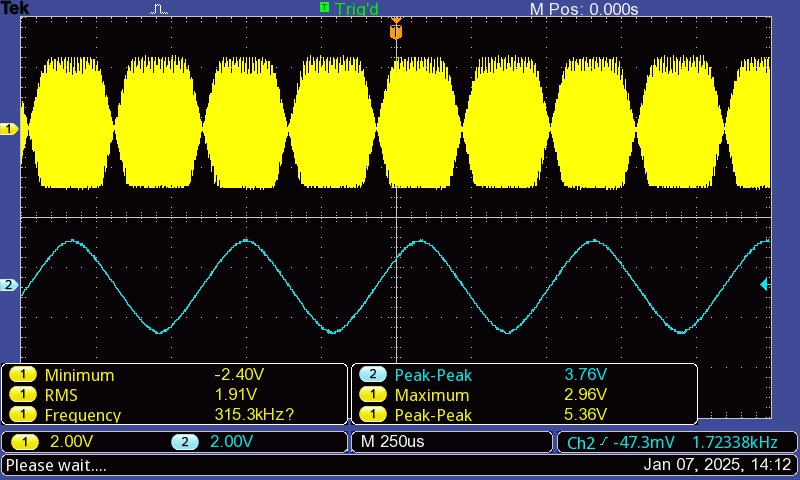
\includegraphics[width=\linewidth]{p8-dsb-mod-msg2.JPG}
        \caption{DSB\-SC; Yellow: Modulated, Blue: Message 2}
        \label{fig:pic8}
    \end{minipage}
    \vspace{1em}
    \begin{minipage}{\linewidth}
        \centering
        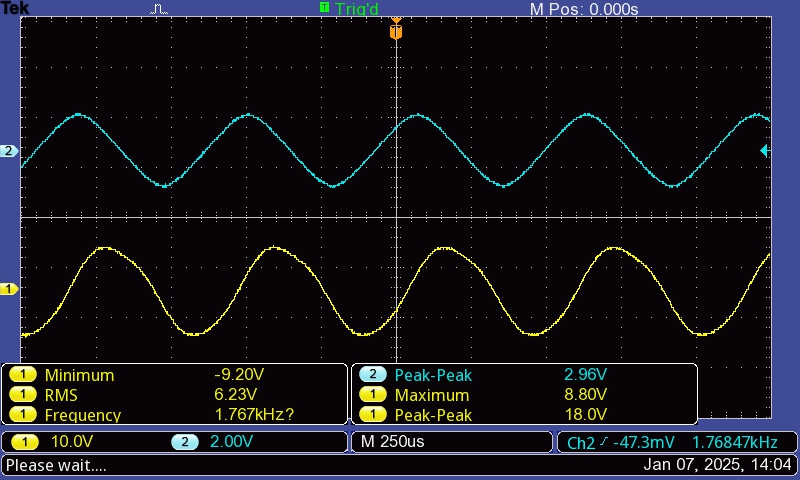
\includegraphics[width=0.4\linewidth]{p9-dsb-msg-Demod.JPG}
        \caption{DSB\-SC; Yellow: Message, Blue: Demodulated Message}
        \label{fig:pic9}
    \end{minipage}
\end{figure}

\subsection*{Matlab Simulation Output}
\addcontentsline{toc}{subsection}{Matlab Output}
\begin{figure}[H]
    \centering
    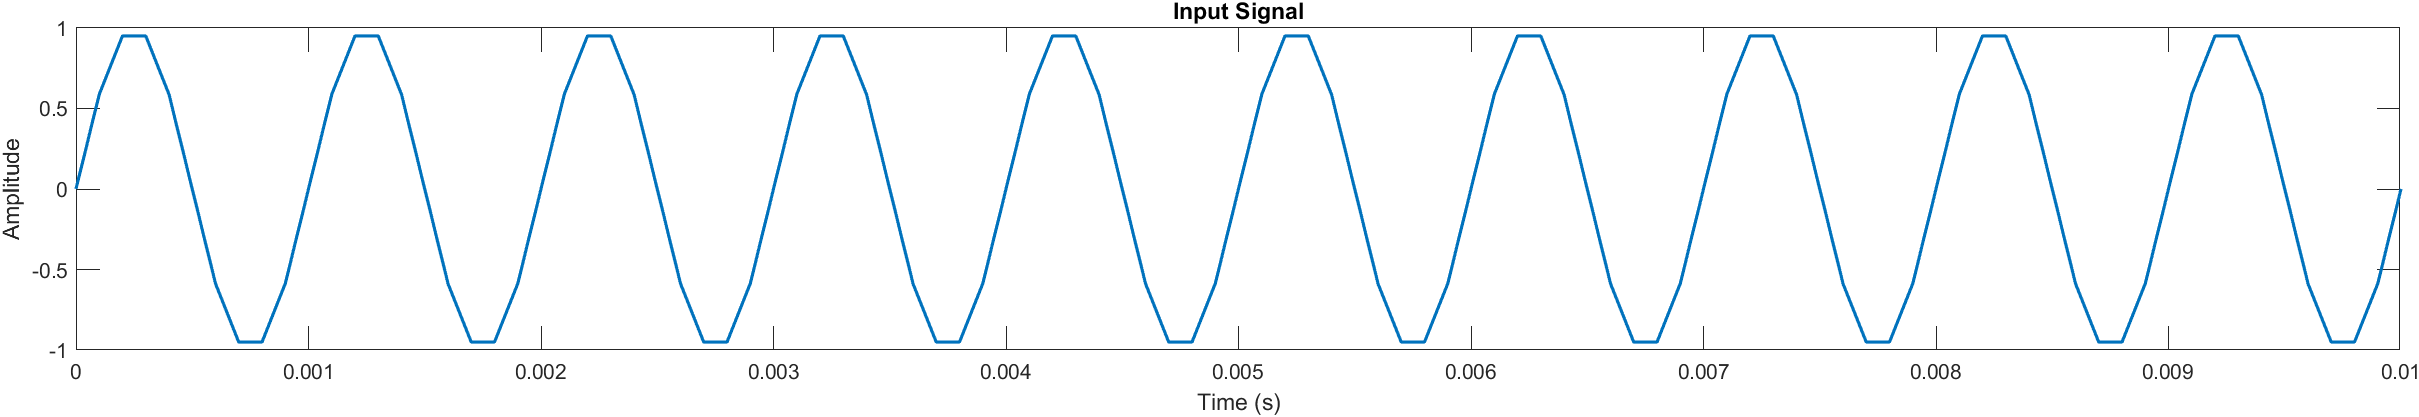
\includegraphics[width=\textwidth]{msg.png}
    \caption{Message Signal}
    \label{fig:img2}
\end{figure}

\begin{figure}[H]
    \centering
    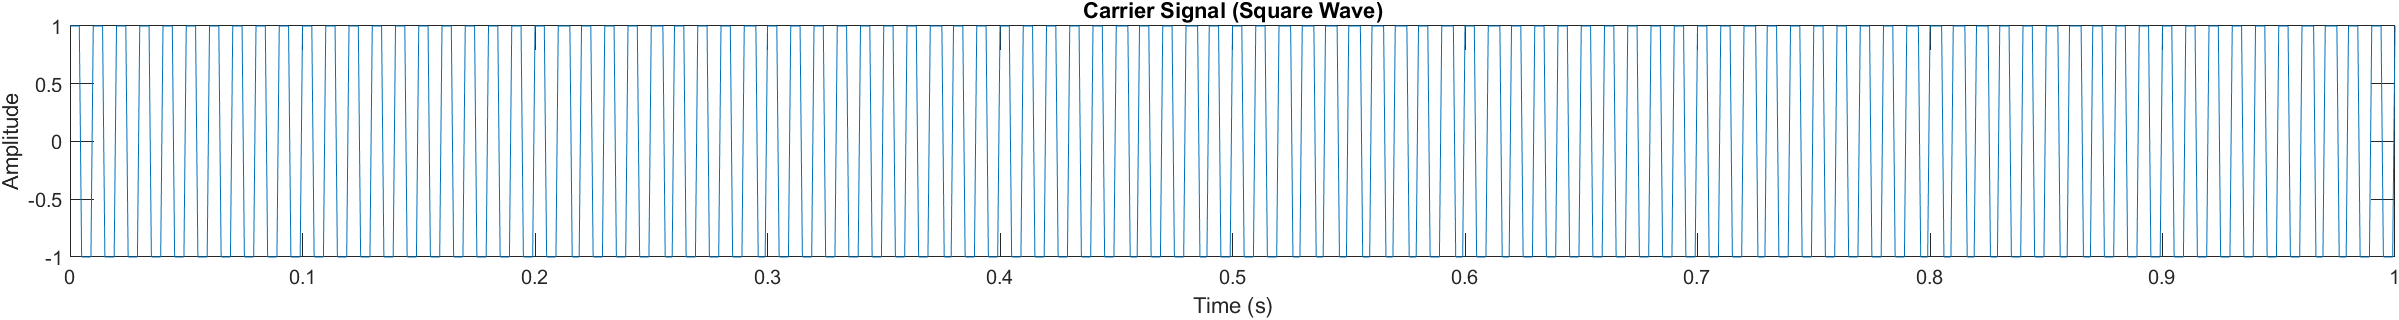
\includegraphics[width=\textwidth]{car.png}
    \caption{Carrier Signal, Square Wave}
    \label{fig:img11}
\end{figure}

\begin{figure}[H]
    \centering
    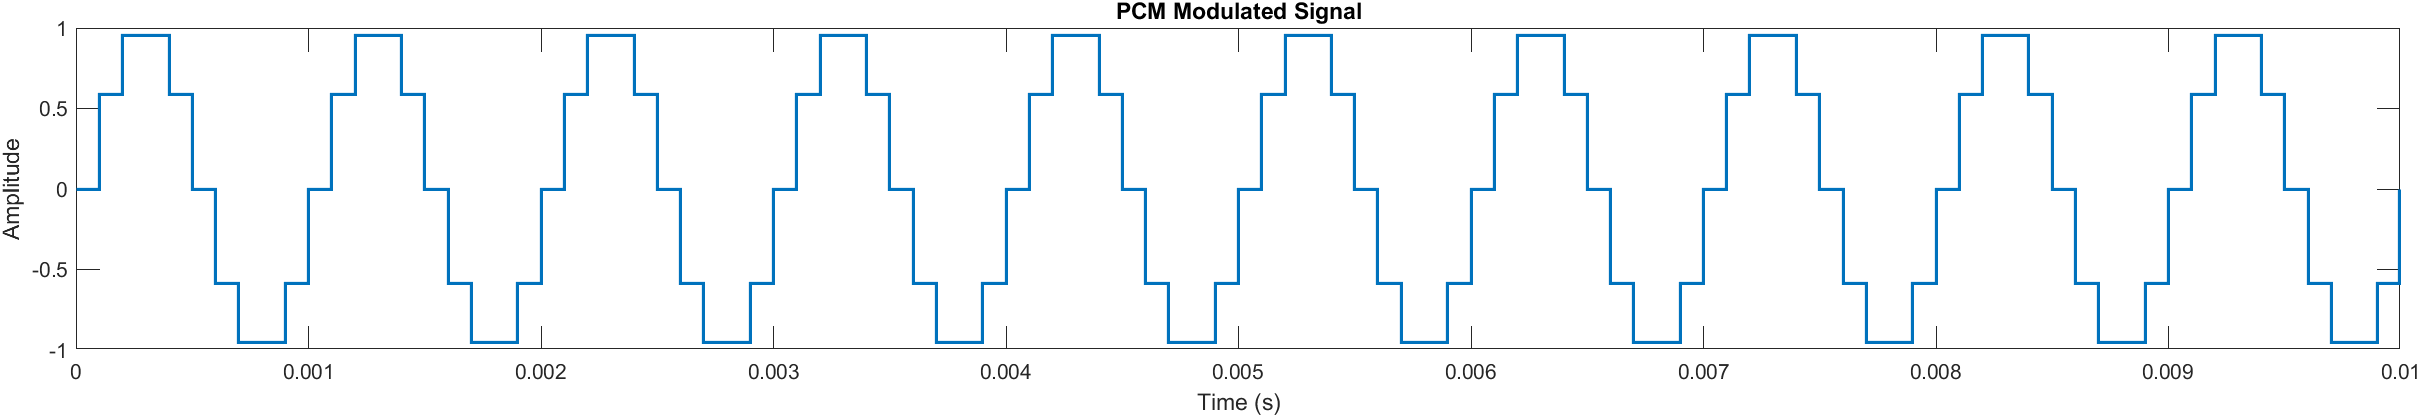
\includegraphics[width=\textwidth]{mod.png}
    \caption{FM Modulated Signal}
    \label{fig:img3}
\end{figure}

\begin{figure}[H]
    \centering
    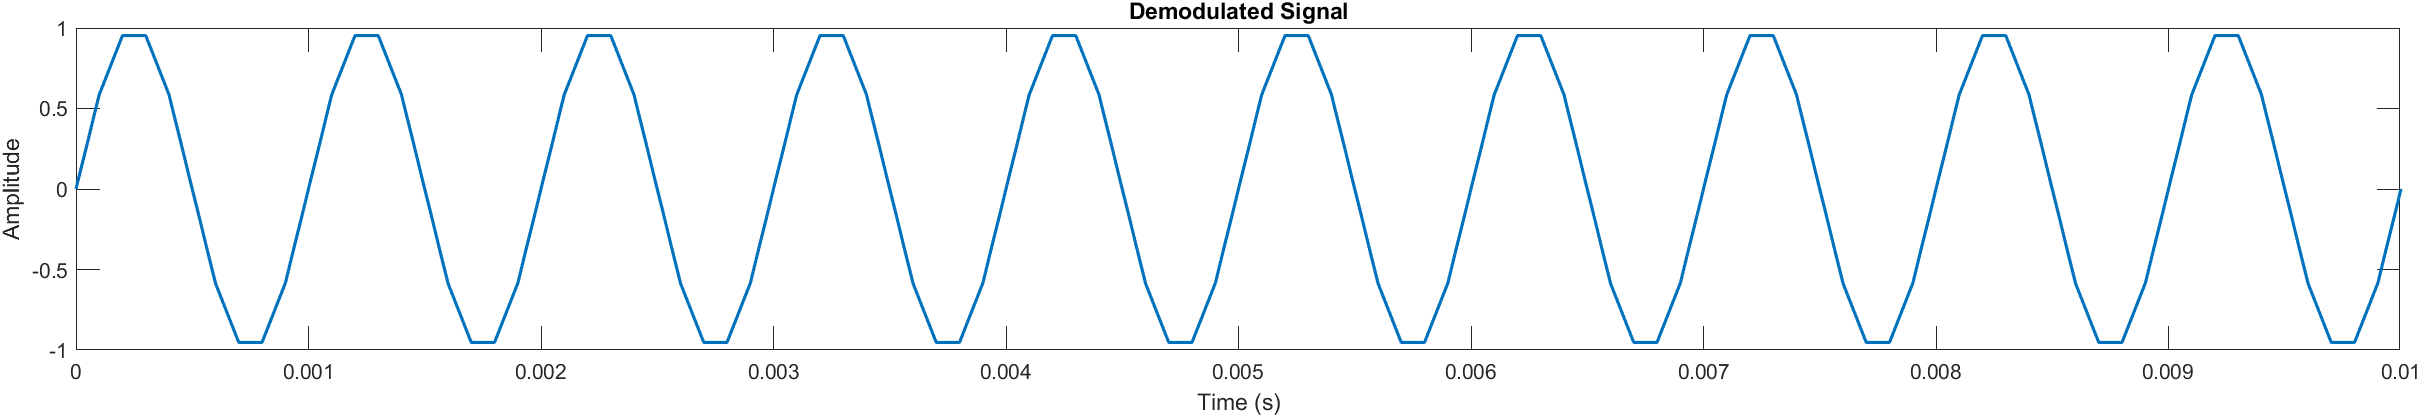
\includegraphics[width=\textwidth]{demod.png}
    \caption{Demodulated Signal}
    \label{fig:img4}
\end{figure}


\section*{Discussion and Conclusion}
\addcontentsline{toc}{section}{Discussion and Conclusion}
The core principles of Pulse Code Modulation (PCM) were effectively demonstrated through the experiment. By adhering to the outlined procedure, the PCM signal and its demodulated output were successfully observed, thereby validating the theoretical concepts of sampling, quantization, and encoding. Notably, significant noise in the PCM and demodulated signals was highlighted, which could be attributed to factors such as faulty connections, external interference, and inaccuracies in sampling or quantization. Addressing these issues through secure connections, functional components, and proper shielding and filtering was deemed crucial.
\\\\
The theoretical understanding was further reinforced by the Matlab simulation, which provided a clear visualization of the PCM process. The simulation output closely aligned with the expected results, confirming the accuracy of the implemented code. Overall, a comprehensive understanding of PCM was offered by the experiment and simulation together, emphasizing the importance of precision in electronic communication systems. Future work could focus on enhancing noise reduction techniques and exploring advanced PCM applications.

\bibliographystyle{IEEEtran}
\renewcommand{\bibname}{References}
\addcontentsline{toc}{section}{References}
\bibliography{ref}

\end{document}
